\documentclass[10pt]{book}
\usepackage[utf8]{inputenc}
\usepackage[T2A]{fontenc}
\usepackage[russian]{babel}
\usepackage{amsmath,amssymb}
\usepackage{jeolm}
\usepackage{jeolm-tourn-limited}
\usepackage{parskip}
\usepackage{graphicx}
\usepackage{multicol}
\pagestyle{empty}

\usepackage{hyperref}
\hypersetup{
    colorlinks,
    citecolor=black,
    filecolor=black,
    linkcolor=black,
    urlcolor=black
}
% \usepackage[a5paper,margin=2em]{geometry}

% \usepackage{pgfpages}
\usepackage{epigraph}
%\pgfpagesuselayout{2 on 1}[a4paper,landscape]

%\def\jeolmleague{7 класс}

\makeatletter

\newcommand{\l@abcd}[2]{\hbox to\textwidth{#1 \dotfill\textbf{ #2}}}

\begin{document}

\begin{center}
	\Huge{\bf 32-я Летняя Многопредметная Школа}\\
	\Large{\bf 7 класс}\\ \vspace{.3cm}
	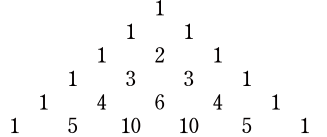
\includegraphics[width=\textwidth]{pasc}
	\begin{multicols}{2}
		Будимир Баев \\
		Владимир Брагин \\
		Надежда Власова \\
		Александр Смирнов \\
	\end{multicols}
\end{center}

\newpage

\begin{center}
На краю \\
Пучины дикой~--- зыбки, а быть может~--- \\
Могилы Мирозданья, где огня\\
И воздуха, материков, морей\\
В помине даже нет, но все они\\
В правеществе зачаточно кишат,\\
Смесившись и воюя меж собой,\\
Пока Творец Всевластный не велит\\
Им новые миры образовать;\\
У этой бездны осторожный Враг,\\
С порога Ада созерцая даль,\\
Обмысливал свой предстоящий путь...
\end{center}

\tableofcontents\newpage

\renewcommand{\@oddhead}{\vbox{\hbox to \textwidth{{\raisebox{1.8mm}{\strut{\small\bfseries Кировская ЛМШ 2016, 7 класс}}\hfil\raisebox{1.8mm}{\strut\bfseries\thepage}}}\hrule}}
\renewcommand{\@evenhead}{\vbox{\hbox to \textwidth{{\raisebox{1.8mm}{\strut\bfseries\thepage}\hfil\raisebox{1.8mm}{\strut{\small\bfseries Кировская ЛМШ 2016, 7 класс}}}}\hrule}}


\addcontentsline{toc}{abcd}{\bf Делимость. 4 июля}
\begin{center}
\textbf{\Large Делимость}\\
%\textit{Профи}\\
\textit{04.07.16}
\end{center}

\epigraph{\it Как зарплату делить будем? Поровну, по-честному, по-братски или по справедливости?}{@shhdup}

\begin{problems}
\item Пусть $a$~--- чётное число, не кратное $4$. Докажите, что разность $a^2 - 4$ делится на $32$.
\item Известно, что $5x+8y-1$ делится на $13$.\\ \textbf{a)} Докажите, что $5x+60y-1$ делится на $13$.\\ \textbf{b)} Найдите остаток от деления $18x-31y$ на $13$. \\ \textbf{c)} Найдите остаток от деления $x-y$ на $13$.
\item Вася написал на доске два числа, перемножил их и получил четырёхзначное число. После этого он заменил буквы на числа, причём разным числам соответствуют разные буквы. В итоге получилось $AB \cdot CD = EEFF$. Докажите, что Вася ошибся.
\item На очень большой и длинной доске записано число $11^{2016}$. Потом вместо этого числа записали сумму его цифр. Затем снова вместо полученного числа записали сумму его цифр. Этот процесс продолжается до тех пор, пока не останется однозначное число. Найдите это число. 
\item На доске записаны два числа: единица и двойка. Каждую минуту Маша умножает два самых больших числа, написанных на доске, прибавляет к ним $1$ и записывает полученное число на доску. Докажите, что Маша никогда не запишет число, делящееся на $4$.
\item Пусть $k>2$~--- нечётное натуральное число. Докажите, что для любого натурального $n$ число $1^{k^n}+2^{k^n}+...+(k-1)^{k^n}$ делится на $k$.
\item Может ли $5^n-1$ делиться на $4^n-1$ при натуральном $n$? 
\item В ряд записана последовательность чисел $a_n$, причём оказалось, что для любого числа, начиная с третьего, справедлива формула $a_n=a_{n-2}+2a_{n-1}$. Оказалось, что первые два члена~--- простые числа. Какое максимальное количество подряд идущих простых чисел может еще встретиться после них?
%\item Можно ли числа $1, 2, 3, . . . , 20$ так расставить в вершинах и серединах ребер куба так, чтобы каждое число, стоящее в середине ребра, равнялось полусумме чисел на концах этого ребра? (не совсем делимость, халява)
% \item Назовем число $n$ \textit{удобным}, если $n^2+1$ делится на $1000001$. Докажите, что среди чисел $1, 2, ..., 1000000$ четное число удобных.
% \item Назовем число совершенно простым, если оно простое и если при любой перестановке его цифр снова получается простое число. Докажите, что в записи абсолютно простого числа не может содержаться более трех различных цифр.
% \item Из трех различных цифр составили шесть различных двузначных чисел (каждая цифра входит в запись по одному разу). Докажите, что если сложить какие-то три из этих чисел и вычесть сумму трех оставшихся, то полученный ответ будет делиться на $18$. 

\end{problems}

\resetproblem
\vspace{1cm}
\newpage
\addcontentsline{toc}{abcd}{\bf Вступительная олимпиада. 4 июля}
\begin{center}
\textbf{\Large Вступительная олимпиада}\\
%\textit{Профи}\\
\textit{04.07.16}
\end{center}


\begin{problems}

\item На острове Мадагаскар есть Холм и Озеро. Глория идет от Холма к Озеру, а навстречу ей от Озера бежит Алекс. Известно, что Глория проходит этот путь за 5 часов, а Алекс всего за час. Через 50 минут после встречи Глории и Алекса Марти также прошел от Озера к Холму, причем это расстояние Марти проходил 1 час 40 минут. Через сколько минут после встречи с Глорией Марти дойдет до Холма, если Глория и Алекс начали движение одновременно? Ответ обоснуйте.

%\item Вася и Петя получили от своих родителей по 100 рублей и решили покататься по городу. Вася катался на маршрутках за 17 и за 10 рублей, а Петя~--- на автобусах за 12 рублей. К вечеру оказалось, что они поездили одинаковое количество раз и потратили одинаковое количество денег. Сколько у них осталось?

%\item На главной диагонали шашечной доски $10\times 10$ стоит 10 шашек (все в разных клетках). За один ход разрешается взять любую пару шашек и передвинуть каждую из них на одну клетку вниз. Можно ли за несколько ходов поставить все шашки на нижнюю горизонталь?

%\item На столе в виде треугольника выложены 28 монет одинакового размера (рис.). Известно, что суммарная масса любой тройки монет, которые попарно касаются друг друга, равна 10  г. Найдите суммарную массу всех 18  монет на границе треугольника.
%\begin{figure}[h!]
%\center{\includegraphics[scale=0.5]{coins.png}}
%\end{figure}\\

\item Натуральные числа от 1 до 20 расставили по кругу в некотором порядке, а затем покрасили в красный цвет те из них, которые являются делителями своего правого соседа. Какое наибольшее количество красных чисел могло получиться?

\item В выпуклом пятиугольнике $ABCDE$ углы $ABC$ и $CDE$ равны, $AB=ED$, $BC=CD$. Докажите, что отрезки $AD$ и $BE$ равны.

\item Пусть $d_1, d_2 , d_3$ и $d_4$~--- наименьшие различные делители натурального числа $n$. Оказалось, что $d_1^2+d_2^2+d_3^2+d_4^2=n$. Чему могло быть равно $n$ (укажите все варианты)?

\item Если в детектор фальшивых монет опустить 5 монет весом $a, b, c, d, e$ граммов, где $a<b<c<d<e$, то он сбросит монеты весом $b$ и $c$ граммов в правую чашу, а остальные в левую. Есть 50 монет попарно различных по весу, они пронумерованы и легко различаются по внешнему виду. Как при помощи детектора определить самую легкую монету?

\item На острове рыцарей (которые говорят только правду) и лжецов (которые всегда
лгут) состоялся шахматный фестиваль. 64 любителя шахмат встали по
одному на клетки большой шахматной доски. После этого каждый сказал:
``{\it Среди людей, стоящих со мной на одной горизонтали, больше лжецов, чем
среди людей, стоящих со мной на одной вертикали}''. Докажите, что
количество рыцарей делится на~8.

\end{problems}

\resetproblem
\vspace{1cm}
\newpage
\addcontentsline{toc}{abcd}{\bf Геометрические неравенства. 5 июля}
\begin{center}
\Large
\textbf{Геометрические неравенства. 05 июля.}
\end{center}  
\large
\begin{enumerate}

\item (тестовая, на знание двух теорем) На стороне $AB$ четырёхугольника $ABCD$ отмечена точка $E$ такая, что $\angle DEA+\angle DBA = 180^{\circ}$. Докажите, что $BC+DE>CD$.

$\textit{Теоретические}$

\item В треугольнике напротив наибольшей стороны угол равен $60^{\circ}$. Чему равны два других угла?

\item На плоскости отмечены точки $A_{1}, A_{2},..., A_{n}$, где $n\geq 3$. Докажите, что $A_{1}A_{2}+A_{2}A_{3}+...+A_{n-1}A_{n}\geq A_{1}A_{n}$. Когда достигается равенство?

\item Отрезки $AC$ и $BD$ пересекаются. Докажите, что $AB+CD<AC+BD$.

\item а) Точки $M$ и $N$ расположены по одну сторону от прямой $\ell$. Постройте на прямой $\ell$ такую точку $K$, чтобы сумма $MK+NK$ была наименьшей. \\
б) Точки $M$ и $N$ расположены по разные стороны от пары параллельных прямых. Постройте на прямых точки $A$ и $B$, так чтобы отрезок $AB$ был перпендикулярен прямым, а сумма отрезков $MA$, $AB$ и $BK$ была наименьшей.\\
в) Точка $M$ лежит внутри острого угла. Постройте на сторонах этого угла точки $A$ и $B$, для которых периметр треугольника $AMB$ был бы наименьшим.

\item а) В треугольнике $ABC$ отмечена точка $T$. Докажите, что $AT+CT<AB+CB$.\\
б) Внутри треугольника $ABC$ расположен треугольник $A_{1}B_{1}C_{1}$. Докажите, что его периметр меньше периметра треугольника $ABC$.\\
в) Внутри выпуклого многоугольника $A_{1}A_{2}...A_{n}$ расположен выпуклый многоугольник $B_{1}B_{2}...B_{m}$. Докажите, что периметр внутреннего многоугольника меньше периметра наружного.

\item В треугольнике $ABC$ отмечена произвольная точка $T$. Докажите, что $AT+BT+CT$ больше полупериметра и меньше периметра треугольника $ABC$. 

$\textit{Более сложные геометрические неравенства}$

\item На стороне $AB$ треугольника $ABC$ отмечена такая точка $D$, что
$AB = CD$. Докажите, что $BC > AD$.

\item Пусть $a, b, c$ — длины сторон треугольника, $m_{a},m_{b},m_{c}$ --- длины опущенных на эти стороны медиан и $p=\frac{a+b+c}{2}$
--- полупериметр данного треугольника. Докажите, что $m_{a}+m_{b}+m_{c}>p$.

\item На основании $AC$ равнобедренного треугольника $ABC$ отметили точку $D$, а на продолжении стороны $AC$ за точку $C$ -- точку $E$ таким образом, что $AD=CE$. Докажите, что $BD+BE>BA+BC$.

\item Отрезки $AA_{1}$ и $BB_{1}$ — биссектрисы треугольника $ABC$. Докажите, что a) $AB_{1} < AB$; б) $A_{1}B_{1} < AB$. 

\item В треугольнике $ABC$ провели биссектрису $CK$, а в треугольнике $CKB$ провели биссектрису $KL$. Прямые $KL$ и $AC$ пересеклись в точке $M$. Известно, что $\angle CAB > \angle BCA$. Докажите, что $AK+KC>AM$.

\end{enumerate}
\resetproblem
\vspace{1cm}
\newpage
\addcontentsline{toc}{abcd}{\bf Графы. 5 июля}
\begin{center}
\Large

\textbf{Графы-1. 05 Июля.}
\end{center}  

\large
\def\q#1.{{\smallskip\bf #1.}}

\q1. На банкете встретились 25 бизнесменов. После банкета каждый из
них пришел домой и послал по подарку каким-то семи из остальных.
Верно ли, что обязательно найдутся два бизнесмена, первый из которых
послал подарок второму, а второй первому~--- нет?


\q2. Чтобы отвести на завтрак, 100 детей построили парами. На обратном 
пути из столовой их снова построили парами, возможно, составленными по-другому. 
При каком наибольшем n наверняка можно выбрать $n$ 
детей, никакие два из них не были в одной паре?

\q3. В стране 12 городов, причем любые два из них соединены дорогой.
10 дорог закрыли на ремонт. Докажите, что из любого города можно
доехать до любого другого по этим дорогам.

\q4. В стране несколько городов, некоторые пары городов соединены
беспосадочными рейсами одной из $N$ авиакомпаний, причем из каждого
города есть ровно по одному рейсу каждой из авиакомпаний. Известно,
что из любого города можно долететь до любого другого (возможно, с
пересадками). Из-за финансового кризиса был закрыт $N-1$ рейс,  но
ни в одной из авиакомпаний не закрыли более одного рейса. Докажите,
что по-прежнему из любого города можно долететь до любого другого.

\q5. В стране 96 городов, из которых 24 -- областные, некоторые пары
городов соединены между собой дорогами (но не более чем одной),
причём любой путь по дорогам между двумя обычными городами, если он
есть, проходит хотя бы через один областной город. Какое наибольшее
количество дорог может быть в этой стране?

\q6. В стране 100 городов, из каждого города выходит хотя бы одна
дорога. Докажите, что можно закрыть несколько дорог так, чтобы
по-прежнему из каждого города выходило не менее одной дороги и при
этом по крайней мере из 67 городов выходило ровно по одной дороге.



\q7. На вечеринку пришло 2016 пар гостей (каждая пара состоит из
мальчика и девочки). Известно, что каждый гость кроме своего
партнера знаком еще хотя бы с одним гостем противоположного пола.
Докажите, что организаторы вечеринки могут раздать всем гостям шляпы
трех цветов так, что у каждого гостя будет хотя бы два знакомых в
шляпах разного цвета.

\q8. На планете 10000 городов, среди которых есть столицы
государств. Некоторые города связаны дорогами так, что любая дорога
соединяет ровно два города, и от любого города до любого другого
можно добраться по дорогам. При этом, чтобы попасть из одной столицы
в другую, нужно проехать не менее 200 дорог. Докажите, что на
планете меньше 100 столиц.

\q9. В кружок записались 15 мальчиков и 15 девочек, причем каждый из
мальчиков знаком хотя бы с тремя девочками. Докажите, что можно
выбрать шестерых мальчиков и двух девочек так, чтобы каждый из
выбранных мальчиков был знаком хотя бы с одной из выбранных девочек.

\resetproblem
\vspace{1cm}
\newpage
\addcontentsline{toc}{abcd}{\bf Разнобой. 5 июля}
\begin{center}
\Large
\textbf{Разнобой-1. 5 июля.}
\end{center}

\begin{enumerate}
\large
\item Сережа написал на доске три натуральных числа, а затем вычислил их попарные НОДы и НОКи. Могла ли сумма шести полученных чисел оказаться равной 1001?

\item Сколько есть прямоугольников из клеток на шахматной доске?

\item В какое наименьшее количество цветов можно покрасить клетки таблицы $4\times4$ (каждая клетка может быть покрашена только в один цвет) так, чтобы для любых различных двух цветов нашлись две клетки, которые покрашены в эти цвета и имеют общую сторону?

\item В треугольнике $ABC$ с $\angle A = 120^{\circ}$ проведены биссектрисы $AA_1$, $BB_1$ и $CC_1$. Прямые $AC_1$ и $BB_1$ пересекаются в точке $T$. Найдите углы треугольника $A_1B_1T$.

\item Существует ли степень двойки, из которой перестановкой цифр (0 ставить на первое место нельзя) можно получить другую степень двойки?


\item Докажите, что уравнение $x^{3}+y^{3}=7\cdot 8^{k}$ не имеет решений в натуральных числах.

\item На плоскости даны $2n$ точек. Два игрока по очереди выбирают по
одной точке до тех пор, пока они не закончатся. Проигрывает тот, у
кого сумма попарных расстояний между выбранными им точками меньше,
чем у соперника. Кто выиграет при правильной игре -- начинающий или
его партнёр? (Все расстояния между данными точками и все суммы
попарных расстояний для разных наборов точек попарно различны.)

\end{enumerate}


\resetproblem
\vspace{1cm}
\newpage
\addcontentsline{toc}{abcd}{\bf Сравнения. 6 июля}
\begin{center}
\Large
\textbf{Сравнения. 06 июля}
\end{center}

{\bf Определение.} Говорят, что целые числа $a,b$ сравнимы по модулю $n$ ($n$ -- натуральное число), если $a-b$ делится на $n$. Обозначается как $a\equiv b (mod \quad n)$

{\bf Свойства. } Пусть $a, b, c, d, e \in \mathbb{Z}, m \in \mathbb{N}$. Если $a \equiv b$ (mod $n$), $c \equiv d$(mod $n$), то:

1) $a+c\equiv b+d$ (mod $n$), $ae\equiv be$ (mod $n$);

2) $ac\equiv bd$ (mod $n$), $a^{m}\equiv b^{m}$ (mod $n$).

3) Если $k$ и $m$ взаимно простые и $ka \equiv kb \quad (mod \quad m)$, то $a \equiv b \quad (mod \quad n)$. (Для доказательства этого свойства пока что ссылаемся на основную теорему арифметики.)

4) Целые числа $a,b$ сравнимы по модулю $n$ тогда и только тогда, когда они имеют одинаковый остаток при делении на $n$ (это не очевидный факт).


\bigskip

{\it О работе со сравнениями, как с уравнениями}

\bigskip


\begin{enumerate}


\item Решите сравнения:\\
а) $5x\equiv 2 \quad  (mod \quad  3)$;\\
б) $3x\equiv 2 \quad (mod \quad  11)$;\\
в) $6x\equiv 1 \quad (mod \quad  13)$;



\item 
а) Пусть $k \in \mathbb{N}$, $n \in \mathbb{N}, 1 \leq n \leq k-1$, $n$ взаимно просто с $k$. Докажите, что существует единственное $m\in \mathbb{N}, 1\leq m \leq k-1$, такое, что $nm\equiv 1$ (mod $k$).

б) Пусть $p\in \mathbb{P},x\in \mathbb{Z}$. Докажите, что если  $x^{2}\equiv 1$ (mod $p$), то либо $x\equiv 1$ (mod $p$), либо $x\equiv -1$ (mod $p$). 

в) ({\bf Теорема Вильсона}) Докажите, что если $p\in \mathbb{P}$, то $(p-1)!\equiv -1$ (mod $p$).


\item Даны натуральные числа $a$, $b$ и $c$ такие, что $ab+9b+81$ и $bc+9c+81$ делятся на $101$. Докажите, что тогда и $ca+9a+81$ тоже делится на 101. 

\bigskip

{\it Перемножаем, складываем.}

\bigskip



\item Натуральные числа $a$ и $b$ таковы, что $ab+1$ делится на $b+2$. Докажите, что $2a > b$.


\item Пусть $a, b, c, d$ и $n$ — натуральные числа, причем $a+b$  и $c+d$ делятся на $n$. Докажите, что $ac-bd$ делится на $n$.


\item а) Докажите, что $a^{n}-b^{n}$ делится на $a-b$.\\
б) Докажите, что при нечётном $n$ $a^n+b^n$ делится на $a+b$.

%$\textit{Якобы практические}$

\item Докажите, что $(2^n-1)^n-3$ делится на $2^n-3$.

\item Вася выписал в тетрадку числа вида $100\ldots 01$ (иными словами, числа вида $10^k+1$), меньшие $10^{2015}$. Докажите, что простых из них не более 1\% от общего числа.




\item Натуральные числа $a$ и $b$ таковы, что $a^{16}+b^{16}$ и $a^{125}+b^{125}$ делятся на 101. Докажите, что $a^{2016}+b^{2016}$ делится на 101.

\item Число $1\underbrace{33...33}_k$ -- простое. Докажите, что $k$ -- нечетное. 

\bigskip

{\it Добавочка.}

\bigskip

\item  Дано четное число $a$. Докажите, что существует бесконечно много нечетных натуральных чисел $n$ таких, что $a^{n} + n$ — составное число.


\item В ряду чисел $1, 501, 751, 876, 438, . . .$ каждое число, кроме первого, равно половине предыдущего, если предыдущее четно, и половине предыдущего числа, увеличенного на 1001, в противном случае. Верно ли, что в этом ряду встретятся все натуральные числа от $1$ до $1000$?


\end{enumerate}
\resetproblem
\vspace{1cm}
\newpage
\addcontentsline{toc}{abcd}{\bf Инвариант. 6 июля}
\begin{center}
\Large
\textbf{Инвариант и не только. 06 июля}
\end{center}


\bigskip
\large
{\it Часть первая.}

\bigskip

\q1. Все клетки доски $8\times 8$ окрашены в белый цвет. Петя перекрасил одну клетку в чёрный. Вася может поменять цвет всех клеток одной строки или столбца. Сможет ли Вася снова сделать всю доску белой?

\q2. На доске написаны числа $1, 5, 10$. Каждую минуту можно любое из чисел заменить на разность суммы двух других и этого числа. Можно ли через некоторое время получить на доске тройку $2013, 2016, 2023$?

\q3. За один ход можно заменить упорядоченную тройку целых чисел
$(p, q, r)$ на тройку $(r+5q, 3r-5p, 2q-3p)$. Существует ли целое число $k$, 
для которого из тройки $(1, 6, 7)$ можно за конечное число шагов получить 
тройку $(k, k+1, k+2)$? 

\q4. В квадрате $4\times 4$ одна крайняя неугловая клетка закрашена в чёрный цвет, а остальные клетки белые. За одну операцию разрешается поменять цвета всех клеток одной линии (будь то строка, столбец или диагональ). Удастся ли сделать доску одноцветной?

\q5. По кругу растут $n$ деревьев. На каждом дереве сидит сова. Каждую минуту какие-то две совы перелетают на соседние деревья, причём одна из них по часовой стрелке, а другая --- против часовой. При каких $n$ все совы смогут оказаться на одном дереве? 



\bigskip

{\it Часть вторая.}

\bigskip

\q6. На доске написаны числа от $1, 2, \ldots 100$. Вася каждую минуту стирает два числа $a$ и $b$ и заменяет их на а)~$a+b$; б)~$ab$; в) $\sqrt{a^2+b^2}$; г) $\frac{ab-1}{a+b+2}$. Докажите, что число, которое останется последним, не зависит от порядка действий.

\q7. С написанными на доске положительными числами разрешается выполнить одну из двух следующих операций:
1)~стереть произвольное число~$x$ и записать два раза число  $\sqrt{x+1}-1$;
2)~стереть два произвольных числа~$x$ и~$y$ и записать число~$x+y+xy$.
Изначально на доске написано число~$a$.
Через несколько операций на доске оказалось написано одно число. Докажите, что оно равно $a$.


\q8. Петя выписал на доске числа от 1 до 100. Каждую минуту Вася стирает с доски два числа, пишет на доску их сумму, а себе в блокнот пишет их произведение. \\
а) Докажите, что сумма чисел  на блокноте после 99 операций не зависит от порядка Васиных действий.\\
б) Чему равна эта сумма?


\q9 . В квадрате $10\times10$ расставлены числа от~1 до~100 следующим образом: в первой строке (слева направо 
по порядку) 1, 2,~\dots 10, во второй~--- 11, 12,~\dots 20,~\dots, в десятой~--- 91, 92,~\dots 100. Разрешается 
взять любой прямоугольник $1\times3$ и сделать следующую операцию: прибавить к крайним числам по~1, а из 
среднего отнять~2, или сделать обратную операцию. Через некоторое время оказалось, что в квадрате опять 
присутствуют все числа от~1 до~100. Докажите, что они расположены на первоначальных местах.
\resetproblem
\vspace{1cm}
\newpage
\addcontentsline{toc}{abcd}{\bf Разнобой. 6 июля}
\begin{center}
\Large
\textbf{Разнобой. 06 июля}
\end{center}

\begin{enumerate}

\item Три простых числа таковы, что квадрат суммы любых двух даёт остаток единицу при делении на третье. Докажите, что какие-то два из чисел равны.


\item $ABCD$~--- выпуклый четырехугольник, в котором $\angle CAD + \angle BCA = 180^{\circ}$ и $AB = BC + AD$. Докажите, что $\angle BAC + \angle ACD = \angle CDA$. 


\item На день рождения к Арсению пришли 12 друзей и расселись за круглым 
столом в ожидании вкусного угощения. После этого перед ними разложили в 
каком-то  порядке карточки с их именами (все имена различны). 
Докажите, что  Арсений может повернуть стол так, чтобы хотя бы двум гостям 
достались карточки с их собственными именами.  

\item Решите в целых числах уравнение $6x+7y=xy-1$.

\item Рассмотрим все треугольники с вершинами в вершинах выпуклого
2016-угольника. Докажите, что любая точка, не лежащая на сторонах таких
треугольников, покрыта четным числом из них.

\item  На бесконечном клетчатом листе двое играют в крестики-нолики по следующим
правилам: первый игрок своим ходом может поставить два крестика, а второй
своим ходом один нолик. Первый игрок выигрывает, если поставит~100 крестиков
подряд. Может ли второй игрок ему помешать?
 

\item Для натурального $n$ введем обозначение 
$$\alpha(n)={(n+1)(n+2)\dots(n+20)\over \hbox{НОК}(n+1, n+2, \dots, n+20)}.$$ 
Докажите, что существуют различные $m, n > 1000$, для которых $\alpha(m)=\alpha(n)$.

\end{enumerate}
\resetproblem
\vspace{1cm}
\newpage
\addcontentsline{toc}{abcd}{\bf Площади. 7 июля}
\begin{center}
\Large
\textbf{Площади. 07 июля.  }
\end{center}


\noindent{\sc Определение.} Каждой фигуре $M$ на плоскости ставится в соответствие
число $S_M$, называемое {\it площадью}, такое, что выполнены следующие
свойства:

1)~$S_M\geq 0$;

2)~Площади равных фигур равны;

3)~Если фигура $M$ состоит из фигур $A$ и $B$, не имеющих общих внутренних
точек, то $S_M = S_A + S_B$;

4)~Площадь квадрата со стороной  $x$ равна $x^2$.


\begin{enumerate}

\item Из того, что площадь квадрата со стороной $x$ равна $x^{2}$ выведите, что площадь прямоугольника со сторонами $a$ и $b$ равна $ab$.

\item а)~Докажите, что площадь прямоугольного треугольника равна половине произведения
его катетов.\\
б)~Докажите, что площадь остроугольного треугольника равна половине произведения
произвольной его стороны на опущенную на эту сторону высоту.\\
в)~Докажите то же самое утверждение для произвольного треугольника.\\
г)~Докажите, что площадь параллелограмма равна произведению
произвольной его стороны на опущенную на эту сторону высоту.\\
д)~Докажите, что площадь трапеции равна произведению полусуммы оснований на высоту.

\item 
Диагонали трапеции $ABCD$ с основаниями $AD$ и~$BC$ пересекаются в точке $O$.
Докажите, что $S_{AOB} = S_{COD}$.

\item а) Докажите, что медиана делит треугольник на два равновеликих.\\
б) Докажите, что медианы треугольника пересекаются в одной точке, делятся точкой пересечения в отношении $2 : 1$, считая от вершины,
и делят треугольник на 6 равновеликих.


\item Каждую сторону треугольника площади $S$ продлили на её длину (см. рисунок). Чему равна площадь большого треугольника?
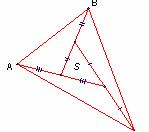
\includegraphics[width=0.2\textwidth]
{square.JPG}

\item Дан выпуклый четырехугольник $ABCD$. На лучах $AB$, $BC$, $CD$ и $DA$ выбраны такие точки $A_1$, $B_1$, $C_1$ и $В_1$, что $AB=A_1B$, $BC=B_1C$, $CD=C_1D$ и $DA=D_1A$. Найдите отношение $S(A_1B_1C_1D_1)/S(ABCD)$.


\item Дан треугольник $ABC$. На луче~$BC$ взята точка~$C_1$.\\
а)~Докажите, что $\frac{S_{ABC_1}}{S_{ABC}} = \frac{|BC_1|}{|BC|}$.\\
б)~Пусть, кроме того, на луче~$BA$ взята точка~$A_1$. Докажите, что
$\frac{S_{A_1BC_1}}{S_{ABC}} = \frac{|BA_1|\cdot |BC_1| }{|BA| \cdot |BC|}$

{\it Вывод: площади треугольников с общим углом относятся, как произведения сторон, этот угол заключающих}

в)~Докажите, что это верно и в случае, когда углы не равны, а дополняют
друг друга до~$180^\circ$.



\item В треугольнике $ABC$ проведена биссектриса $BL$. Докажите, что $\frac{|AL|}{|CL|}=\frac{|AB|}{|CB|}$.

\item а)~Две параллельные прямые пересекают стороны угла с вершиной~$O$ в точках
$A$, $B$ и $A_1$, $B_1$ соответственно. Докажите, что~$\frac{|OA|}{|OB|} = \frac {|OA_1|}{|OB_1|}$.\\
б)~({\bf Теорема Фалеса}) Три параллельные прямые пересекают стороны угла с вершиной~$O$ в точках
$A$, $B$, $C$ и $A_1$, $B_1$, $C_1$ соответственно. Докажите, что~$\frac{|AB|}{|BC|} = \frac {|A_1B_1|}{|B_1C_1|}$.\\
в) ({\bf Обратная теорема Фалеса}) Две прямые пересекли стороны угла с вершиной $O$ в точках $A_{1},B_{1}$ и $A_{2}, B_{2}$ соответственно. Оказалось, что $\frac{|OA|}{|OB|} = \frac {|OA_1|}{|OB_1|}$. Докажите, что эти прямые параллельны.


\end{enumerate}
\resetproblem
\vspace{1cm}
\newpage
\addcontentsline{toc}{abcd}{\bf Треугольник Паскаля. 7 июля}
\begin{center}
\Large
\textbf{Подсчет числа способов. Треугольник Паскаля. 07 июля.}
\end{center}  

\def\q#1.{{\smallskip\bf #1.}}
\q0. a) Имеется $m$ белых и $n$ черных шаров, причем  $m > n$.
Сколькими способами можно все шары разложить в ряд так, чтобы
никакие два черных шара не лежали рядом? \\
b) Cколькими способами можно рассадить m разноцветных попугаев по n клеткам так, чтобы в каждой сидели один или два попугая?\\
c) Сколькими способами можно выбрать $k$ различных подмножеств $n$-элементного множества?\\
d) Сколькими способами можно выбрать $k$ непересекающихся множеств из $n$ элементного множества?

\medskip

{\bf Напоминание.} Число способов выбрать из~$n$ предметов
произвольные~$k$ равно~$\frac{n!}{(n-k)!k!}$ и обозначается~$C_n^k$.

\q1. Докажите следующие равенства: \\
 a) $kC_n^k=nC_{n-1}^{k-1}$\\
 b) $C_n^k=C_{n-1}^k + C_{n-1}^{k-1}$;\\
 c) $C_r^mC_m^k=C_r^kC_{r-k}^{m-k}$

\q2. ({\bf Бином Ньютона}) Докажите формулу
$$(x+y)^n=\sum_{k=0}^nC_n^kx^ky^{n-k}.$$
(коэффициенты $C_n^k$ называются {\it биномиальными}.)

\q3. Найдите следующие суммы
\begin{equation*}
a) \sum_{k=0}^n C_n^k; \quad b) \sum_{k=0}^n 2^kC_n^k; \quad c)
\sum_{k=0}^n (-1)^kC_n^k; \quad d) \sum_{k=0}^n kC_n^k \quad
\end{equation*}
%над последним пунктом засядут


\q4. Дана клетчатая доска размера $n \times m$, в левом нижнем углу
которой стоит фишка. За один ход можно переместить фишку на одну
клетку вверх или вправо. Сколькими способами можно добраться до
правого верхнего угла доски?



\medskip

{\bf Опр.} {\it Треугольник Паскаля}~--- бесконечная таблица
биномиальных коэффициентов, имеющая треугольную форму. В этом
треугольнике на вершине и по бокам стоят единицы. Каждое число равно
сумме двух расположенных над ним чисел.

\medskip

\q5. Докажите, что каждое число $a$ в треугольнике Паскаля,
уменьшенное на~1, равно сумме всех чисел, заполняющих
параллелограмм, ограниченный теми правой и левой диагоналями, на
пересечении которых стоит число $a$ (сами эти диагонали в
рассматриваемый параллелограмм не включаются).

\q6. Дан треугольник Паскаля из $n$ строк. Найдите сумму всех его
элементов.

\q7. {\it Диагональю} треугольника Паскаля называется множество
чисел, расположенных на прямой, параллельной его стороне. Найдите
сумму чисел, стоящих на $k$-ой диагонали треугольника из $n$ строк.

\q8. Докажите равенство:
$1^2+2^2+\ldots+k^2=C_{k+1}^2+2(C_k^2+C_{k-1}^2+\ldots+C_2^2)$.

\q9. Докажите, что не существует таких натуральных чисел $x$, $y$,
$z$, $k$, что $x^k + y^k = z^k$  при условии  $x < k,  y < k$.

\q10. В левом столбце и нижней строке таблицы $11 \times 11$ лежат
фишки~--- всего $2^{15}$ фишек. За один ход разрешается выбрать две
граничащие по углу клетки, снять с них по фишке и добавить фишку в
клетку, имеющую общую сторону с выбранными. Можно ли добиться того,
чтобы хотя бы одна фишка попала в правый верхний угол?

\resetproblem
\vspace{1cm}
\newpage
\addcontentsline{toc}{abcd}{\bf Индукция. 9 июля}
\begin{center}
\Large
\textbf{Индукция. 9 июля. }
\end{center}  

\bigskip
\large
{\bf Можно сдавать только решения с помощью метода математической  индукции, даже если очень хочется по-другому.}

\bigskip

\q1. Докажите, что $1^2+3^2+\ldots +(2k-1)^2 = \frac{k(4k^2-1)}{3}$.

\quad

\q2. Определим число $n?$ ("эн вопросиал") следующим образом: $1? = 1$, 
$n?={n\over (n-1)?}$ для всех $n>1$. Докажите, что $n?\times n!$ -- 
квадрат натурального числа.

\quad


\q3. Для каких натуральных $n$ выполнено неравенство $2^n>n^3$?


\quad




\q4. Обозначим за $P(n)$ произведение всех простых чисел, меньших $n$. Докажите, что если $n>3$, то $P(n)>n$.

 
\quad




\q5. Вася написал на $n!$ бумажках все возможные последовательности, содержащие числа от 1 до $n$ по одному разу. Докажите, что можно выложить бумажки по кругу так, чтобы последовательности, написанные на соседних бумажках, отличались лишь перестановкой двух соседних чисел. 


\quad


\q6. В военную часть приехало $n$ незнакомых друг с другом новобранцев. Прапорщик сообщил каждому новобранцу натуральное число так, что сумма всех $n$ чисел равна $2n-2$. Докажите, что можно познакомить некоторых из них друг с другом так, чтобы каждый 
новобранец имел количество знакомых, равное числу, которое ему сообщил прапорщик.

\quad

\q7. На ежегодный слет-проверку съехались 100 бригад СЭС и поселились в 100 корпусах. Каждая бригада хочет проверить три корпуса (заранее сообщая номера начальнику лагеря) и тут же уехать из лагеря. Докажите, что начальник может составить расписание проверок так,  чтобы никакую бригаду не проверяли более трех раз (проверять пустые корпуса можно сколько угодно раз).

\quad




\q8. В стране $n$ городов. Каждые два города соединены дорогой. По указу Парламента Министерству транспорта необходимо вести учёт всех циклических туристических маршрутов. Докажите, что министерство транспорта может так ввести одностороннее движение на дорогах, чтобы из любого города можно было доехать до любого другого и для каждого $k\leqslant n$ циклических маршрутов длины $k$ было ровно $n-k+2$ (то есть, чтобы учёта нужно было вести как можно меньше). 

\quad

\q9. В каждой клетке таблицы $1000\times 1000$ стоит ноль или единица. Докажите, что можно либо вычеркнуть 990 строк так, что каждом столбце будет хотя бы одна невычеркнутая единица, либо вычеркнуть 990 столбцов так, что в каждой строке будет хотя бы один невычеркнутый ноль.

\resetproblem
\vspace{1cm}
\newpage
\addcontentsline{toc}{abcd}{\bf Геометрический разнобой. 9 июля}
\begin{center}
\Large
\textbf{Геометрический разнобой. 9 июля. }
\end{center}  

\bigskip

\q1. а) Докажите, что на первом рисунке площадь закрашенной части равна площади незакраменной.


б) Докажите, что на втором рисунке площадь закрашенной дважды части равна площади незакрашенной совсем.

\begin{center}

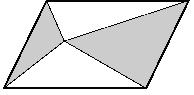
\includegraphics[width=0.4\textwidth]{2b.JPG}
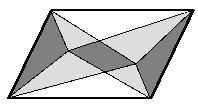
\includegraphics[width=0.4\textwidth]{2d.JPG}
\end{center}

% Про лемму о линолеуме

\q2. На сторонах $AB$, $BC$ и $CA$ треугольника $ABC$, площадь которого равна $S$, выбраны точки $C_1$, $A_1$ и $B_1$ так, что $AC_1 = 2C_1B$, $BA_1=2A_1C$ и $CB_1=2B_1A$. Чему равна площадь треугольника $A_1B_1C_1$? 

% на площадь и отношение оснований

\q3. Дан равносторонний треугольник $ABC$ и точка $X$ внутри. Докажите, что сумма расстояний от точки $X$ до сторон треугольника не зависит от точки $X$
% на площадь

\q4т. а) На сторонах прямоугольного треугольника во внешнюю сторону построены квадраты. Докажите, что площади тёмных треугольничков на рисунке равны.\\

\begin{center}
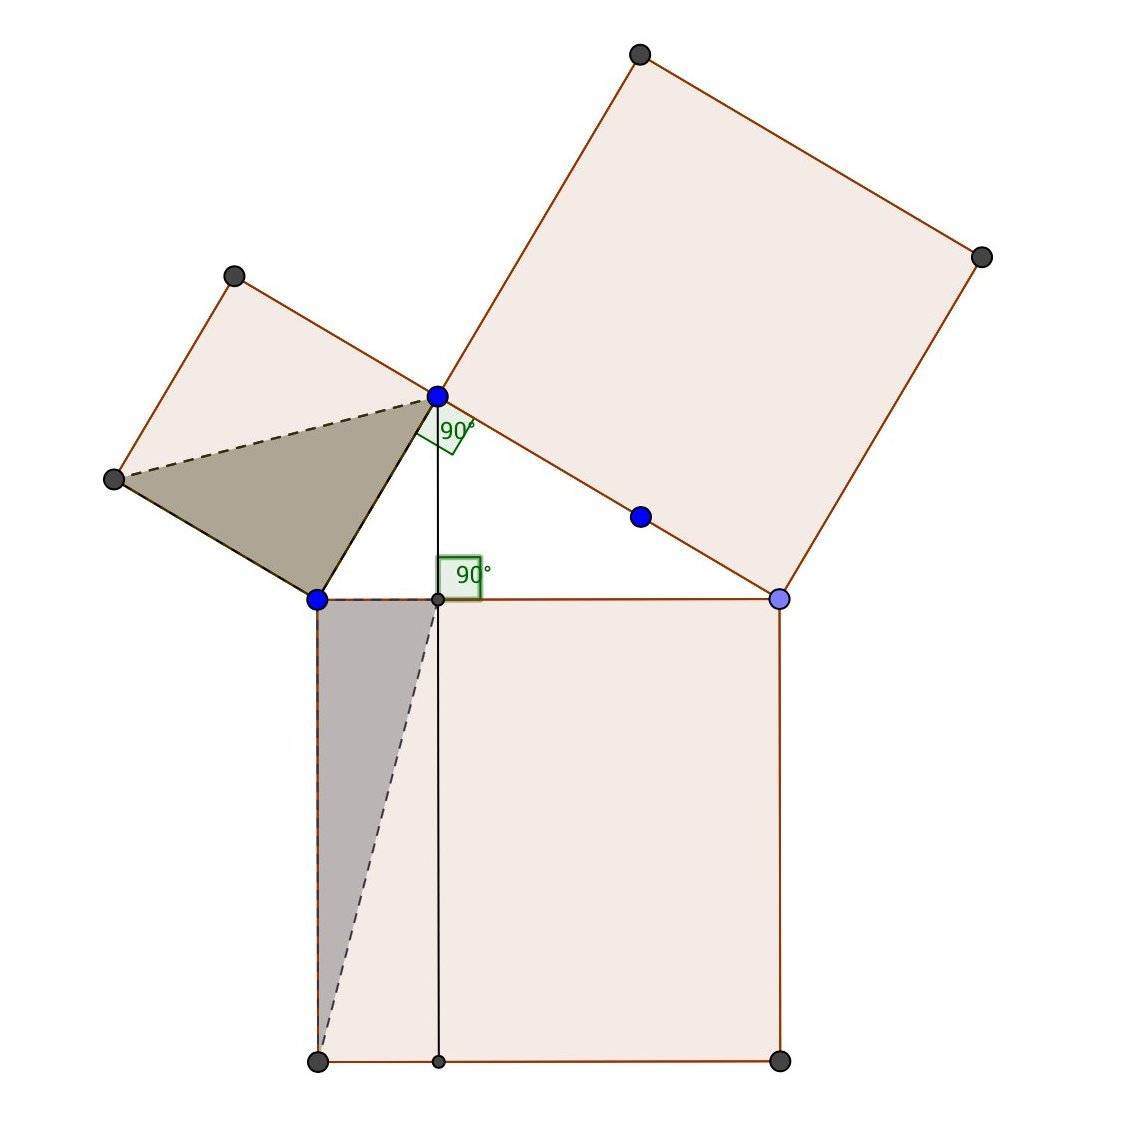
\includegraphics[width=0.4\textwidth]{pifagor.jpg}
\end{center} 


б) Выведите отсюда теорему Пифагора.

%Теорема Пифагора 


\q5т. а) Диагонали четырёхугольника $ABCD$ перпендикулярны. Докажите, что $AB^2+CD^2=AD^2+BC^2$.


б) Докажите, что если в четырёхугольнике $ABCD$ выполнено $AB^2+CD^2=AD^2+BC^2$, то его диагонали перпендикулярны. 
%На теорему Пифагора


\q6т. Треугольники~$ABC$ и~$A_1B_1C_1$ таковы, что $AB=A_1B_1$,
\quad $BC=B_1C_1$
и~$\angle A = \angle A_1$. Докажите, что либо эти треугольники равны, либо
$\angle C + \angle C_1 = 180^{\circ}$.
% четвёртый признак

\q7. На гипотенузе~$AC$ прямоугольного треугольника $ABC$ выбрали точку~$D$
такую, что $BC=CD$. На катете~$BC$ выбрали такую точку~$E$, что $DE=CE$.
Докажите, что $AD+BE=DE$.
% На равенство треугольников с доп построением


\q8.  В треугольнике $ABC$ \quad $AB<AC$. Прямая, проходящая через вершину~$B$ параллельно~$AC$, пересекает
биссектрису внешнего угла~$A$ в точке~$D$. Прямая, проходящая через вершину~$C$ параллельно~$AB$, пересекает
эту биссектрису в точке~$E$. На стороне~$AC$ выбрана точка~$F$ так, что $FC=AB$.  Доказать, что $DF=FE$.

% На равенство треугольников с доп построением


\q9. Внутри треугольника $ABC$ отмечена точка $M$, так что при этом
$\angle  BAM=\angle ABC$, $\angle AMB=100^{\circ}$,
$\angle ACB=70^\circ$. Докажите, что $BM<AC$.

\resetproblem
\vspace{1cm}
\newpage
\addcontentsline{toc}{abcd}{\bf Алгоритм Евклида. 9 июля}
\begin{center}
\Large

\textbf{НОД. Алгоритм Евклида. 09 Июля.}
\end{center}  

\large
\def\q#1.{{\smallskip\bf #1.}}

\bigskip
\large

\begin{definition}
\emph{Алгоритм Евклида.}

Пусть a и b — целые числа, не равные одновременно нулю, и последовательность чисел
$a > b > r_1 > r_2 > r_3 > r_4 > \cdots > r_n$
определена тем, что каждое $r_k$~-- это остаток от деления предпредыдущего числа на предыдущее, а предпоследнее делится на последнее нацело, то есть \\
$a = bq_0 + r_1 \\
b = r_1q_1 + r_2 \\
r_1 = r_2q_2 + r_3 \\
\cdots \\
r_{k-2} = r_{k-1} q_{k-1} + r_k \\
\cdots \\
r_{n-2} = r_{n-1}q_{n-1}+ r_n \\
r_{n-1} = r_n q_n$ \\
Тогда $(a,b)=r_n$.
\end{definition}



\q0т. а) Докажите, что для любых целых $a, b, k$ выполнено $(a, b) = (b, a-kb)$.\\
 б) Докажите, что алгоритм Евклида действительно выдаёт наибольший общий делитель двух чисел.\\





\q1. При каких $n$ дробь $\frac{n^2+2n+4}{n^2+n+3}$ несократима?

\q2. Докажите, что $(a^{n}-1,a^{m}-1)=a^{(n,m)}-1$.

\q3. Какое наибольшее значение может принимать $(15a+16b, 16a-15b)$?

\q4. a) Найдите $(f_{n},f_{m})$, где $f_{k}=2^{2^{k}}+1$ - числа Ферма. \\ 
b) Докажите, что число $2^{2^{k}}-1$ имеет хотя бы $k$ различных простых делителей. \\
с) Из этого докажите, что простых чисел бесконечно много.

\q5т. {\bf Теорема о линейном представлении НОД.} Докажите, что существуют такие целые $x$ и $y$ , что $xa+yb=(a,b)$

\q6. Пусть $ab$ делится на $c$, $(a,c)=1$. Докажите, что $b$ делится на $c$. (Основной теоремой арифметики, разумеется, пользоваться нельзя.)

\q7т. {\bf Основная теорема арифметики.} Докажите, что каждое натуральное число $n>1$ можно единственным способом представить в виде $n=p_{1}^{d_{1}}\cdot \dots \cdot p_{k}^{d_{k}}$, где $ p_{1}<\dots <p_{k}$ — простые числа, а $d_{1}\cdot \dots \cdot d_{k}$ - натуральные числа.

\q8. По бесконечной шахматной доске ходит $(m,n)$-мамонт, который за один ход может сдвинуться на $m$ клеток по горизонтали или вертикали, а затем - на $n$ клеток в перпендикулярном направлении. При каких $m, n$ $(m,n)$-мамонт сможет из любой клетки доски попасть в любую другую?

\q9. Аня нашла себе интересное занятие. Она написала на доске две единички, потом между ними написала их сумму. Ее это так захватило, что она продолжила: брала ряд чисел, который у нее получился на предыдущем шаге, и между двумя соседними числами писала их сумму (старые числа при этом не стирала). Докажите, что любое $n>1$ она написала ровно $\varphi(n)$ раз.  Напомним, что $\varphi(n)$ -- это количество чисел, не превосходящих $n$ и взаимно простых с $n$.

\resetproblem
\vspace{1cm}
\newpage
\addcontentsline{toc}{abcd}{\bf Малая теорема Ферма. 10 июля}
\begin{center}
\Large
\textbf{Теория чисел. Малая теорема Ферма. 10 июля.}
\end{center}

{\large
\q1т. а)~Пусть $a,b \in \mathbb Z$ и~$p \in \mathbb P$. Докажите,
что~$(a+b)^p \equiv a^p+b^p \pmod{p}$.

б)~Выведите отсюда по индукции { \it малую теорему Ферма}: если $p\in \mathbb{P}, a\in \mathbb{Z}$ и $a$ не делится на $p$, то $a^{p-1}\equiv 1$ (mod $p$).




\q2т.  Пусть $a \in \mathbb{Z}, p \in \mathbb{P}$ и $a$ не делится на $p$. Рассмотрим следующий ориентированный граф: вершины графа — числа от 1 до $p-1$; из числа $x$ ведет ориентированное ребро в число $y$, если $ax \equiv y$ (mod $p$). 

а) Докажите, что этот граф является объединением нескольких циклов одинаковой длины.

б) Выведите из этого { малую теорему Ферма}.

\q3т. Возьмём натуральное число $a$, которое не делится на простое число $p$. 


а) Докажите, что среди остатков $a, 2a, 3a, \ldots (p-1)a$ есть все ненулевые остатки по модулю~$p$. 


б) Перемножив всё это, выведите малую теорему Ферма. 

\q4. Пусть $p$ и $q$ --- различные простые числа. Докажите, что $p^q+q^p \equiv p+q \pmod  {pq}$.


\q5. Какой остаток даёт число $42^{42^{42}}$ при делении на 2017?

\q6.  Дано простое число $p$. Докажите, что $2^{2^p}-4 $ делится на $2^p-1$.

\q7. Докажите, что если $a^{15}-1$ делится на 29, то и $a-1$ делится на 29.

\q8. Какие остатки может давать число $a^{50}$ при делении на 101?}

\resetproblem
\vspace{1cm}
\newpage

\end{document}